\documentclass[margin=0px]{article}

\usepackage{listings}
\usepackage[utf8]{inputenc}
\usepackage{graphicx}
\usepackage{float}
\usepackage[a4paper, margin=1in]{geometry}
\usepackage{amsthm}
\usepackage{amssymb}
\usepackage{amsmath}

\newenvironment{tetel}[1]{\paragraph{#1}}{}
\renewcommand{\figurename}{ábra}
\makeatletter
\renewcommand\paragraph{%
	\@startsection{paragraph}{4}{0mm}%
	{-\baselineskip}%
	{.5\baselineskip}%
	{\normalfont\normalsize\bfseries}}
\makeatother

\usepackage{pdfpages}

% A dokument itt kezdődik
\title{Záróvizsga tételsor \\ \large 7. Programozás}
\date{}
\author{Ancsin Ádám}

\begin{document}
	\maketitle
	
	\begin{tetel}{Programozás}
			Egyszerű programozási feladat megoldásának lépései (specifikálás, tervezés, megvalósítás, tesztelés). Az adattípus fogalma (típusspecifikáció, műveletek, reprezentáció, invariáns, implementáció). A visszavezetés módszere. A felsoroló típus specifikációja. Felsorolóra megfogalmazott programozási tételek (összegzés, számlálás, maximum kiválasztás, feltételes maximumkeresés, lineáris keresés, kiválasztás). Nevezetes gyűjtemények (intervallum, tömb, sorozat, halmaz, szekvenciális inputfájl) felsorolói.
	\end{tetel}
	
	
	\section{Egyszerű programozási feladat megoldásának lépései}
	\subsection{Bevezetés}
	Egy programozási feladat megoldása a kódoláson túl jó néhány tevékenységet tartalmaz.
	Az első teendő a feladat pontos meghatározása, a specifikáció. Ez a feladat szöveges és formalizált, matematikai leírásán (a specifikáció ún. szűkebb értelmezésén) túl tartalmazza a megoldással szemben támasztott követelményeket, környezeti igényeket is (ami a specifikáció ún. tágabb értelmezése).
	
	A specifikáció alapján meg lehet tervezni a programot, elkészülhet a megoldás algoritmusa és az algoritmus által használt adatok leírása. Az algoritmus és az adatszerkezet finomítása egymással párhuzamosan halad, egészen addig a szintig, amelyet a programozó ismeretei alapján már könnyen, hibamentesen képes kódolni. Gyakran előfordul, hogy a tervezés során derül fény a specifikáció hiányosságaira, így itt visszalépésekre számíthatunk.
	
	Az algoritmusírás után következhet a kódolás. Ha a feladat kitűzője nem rögzítette, akkor ez előtt választhatunk a megoldáshoz programozási nyelvet. A kódolás eredménye a programozási nyelven leírt program.
	
	A program első változatban általában sohasem hibátlan, a helyességéről csak akkor beszélhetünk, ha meggyőződtünk róla. A helyesség vizsgálatának egyik lehetséges módszere a tesztelés. Ennek során próbaadatokkal próbáljuk ki a programot, s az ezekre adott eredményből következtetünk a helyességre. (Ne legyenek illúzióink afelől, hogy teszteléssel eldönthető egy program helyessége. Hisz hogy valójában helyes-e a program – sajnos – nem következik abból, hogy nem találtunk hibát.)
	
	Ha a tesztelés során hibajelenséggel találkozunk, akkor következhet a hibakeresés, a hibajelenséget okozó utasítás megtalálása, majd pedig a hibajavítás. A hiba kijavítása több fázisba is visszanyúlhat. Elképzelhető, hogy kódolási hibát kell javítanunk, de az is lehet, hogy a hibát már a tervezésnél követtük el. Javítás után újra tesztelni kell, hiszen – legyünk őszinték magunkhoz!– nem kizárt, hogy hibásan javítunk, illetőleg – enyhe optimizmussal állítjuk:– a javítás újabb hibákat fed fel, ...
	
	E folyamat végeredménye a helyes program. Ezzel azonban még korántsem fejeződik be a programkészítés. Most következnek a minőségi követelmények. Egyrészt a hatékonyságot kell vizsgálnunk (végrehajtási idő, helyfoglalás), másrészt a kényelmes használhatóságot. Itt újra visszaléphetünk a kódolási, illetve a tervezési fázisba is. Ezzel elérkeztünk a jó programhoz.
	
	\subsection{Specifikáció}
	A programkészítés menetének első lépése a feladat meghatározása, precíz "újrafogalmazása". Milyen is legyen, mit várjunk el tőle? Nézzünk meg néhány – jónak tűnő – követelményt egyelőre címszavakban! (A továbbiakban a specifikáció szűkebb értelmezéséről lesz szó.) A specifikáció legyen:

	\begin{itemize}
		\item helyes, egyértelmű, pontos, teljes
		\item rövid, tömör, ami legegyszerűbben úgy érhető el, hogy ismert formalizmusokra építjük
		\item szemléletes, érthető (amit időnként nehezít a formalizáltság) 
	\end{itemize}
	
	A specifikáció első közelítésben lehetne a feladatok szövege. Ez azonban több problémát vethet fel:
	
	\begin{itemize}
		\item mi alapján adjuk meg a megoldást
		\item mit is kell pontosan megadni?
	\end{itemize}
	
	Például az a feladat, hogy adjuk meg N ember közül a legmagasabbat. A legmagasabb ember megadása mit jelent? Adjuk meg a sorszámát, vagy a nevét, vagy a személyi számát, vagy a magasságát, esetleg ezek közül mindegyiket?
	Tanulságként megállapíthatjuk, hogy a specifikációnak tartalmaznia kell a bemenő és a kimenő adatok leírását.
	
	\begin{verbatim}
	Bemenet: 
	    N : az emberek száma,
	    A : a magasságukat tartalmazó sorozat.
	
	Kimenet:
	    MAX : a legmagasabb ember sorszáma.
	\end{verbatim}

	
	Tudjuk-e, hogy a bemenő, illetve a kimenő változók milyen értéket vehetnek fel? Például az emberek magasságát milyen mértékegységben kell megadni? Az eredményül kapott sorszám milyen érték lehet: 1-től sorszámozunk, vagy 0-tól? Megállapíthatjuk tehát, hogy a specifikációban a bemeneti és a kimeneti változók értékhalmazát is meg kell adnunk.
	
	\begin{verbatim}
	Bemenet:
	    N : az emberek száma, természetes szám;
	    A : a magasságukat tartalmazó sorozat, egész számok, amelyek a magasságot
	        centiméterben fejezik ki (a sorozatot 1-től N-ig indexeljük).
	Kimenet: 
	    MAX : a legmagasabb ember sorszáma, 1 és N közötti természetes szám.
	\end{verbatim}
	
	Most már a bemenő és a kimenő változók értékhalmazát pontosan meghatároztuk, csupán az a probléma, hogy a feladatban használt fogalmakat és az eredmények kiszámítási szabályát nem definiáltuk. A specifikációnak tehát tartalmaznia kell a feladatban használt fogalmak definícióját, valamint az eredmény kiszámítási szabályát. Itt lehetne megadni a bemenő adatokra vonatkozó összefüggéseket is. A bemenő, illetve a kimenő adatokra kirótt feltételeket nevezzük előfeltételnek, illetve utófeltételnek. Az előfeltétel nagyon sokszor egy azonosan igaz állítás, azaz a bemenő adatok értékhalmazát semmilyen "külön” feltétellel nem szorítjuk meg.
	
	\begin{verbatim}
	Bemenet: 
     	N : az emberek száma, természetes szám,
     	A : a magasságukat tartalmazó sorozat, egész számok, 
        	amelyek a magasságot centiméterben tartalmazzák (a sorozatot 1-tol N-ig indexeljük).
	Kimenet:	
     	MAX : a legmagasabb ember sorszáma, 1 és N közötti természetes szám.
	
	Elofeltétel: 
    	A[i]-k pozitívak.
	
	Utófeltétel: 	
	    MAX olyan 1 és N közötti szám, amelyre A[MAX] nagyobb vagy egyenlo, 	
	    mint a sorozat bármely eleme (az 1. és az N. között).
	\end{verbatim}
	
	Újabb probléma merülhet fel bármelyik feladattal kapcsolatban: az eddigiek alapján a "várttól” lényegesen különböző – nyugodtan állíthatjuk: "banális” –, az elő- és utófeltételnek megfelelő megoldást is tudunk készíteni. 
	
	Itt persze arról a hallgatólagos (tehát még meg nem fogalmazott, ki nem mondott) feltételezésről van szó, hogy a bemeneti változók értéke nem változik meg. Ez sajnos nem feltétlenül igaz. A probléma megoldására kétféle utat követhetünk (a későbbiekben mindkettőt alkalmazni fogjuk):
	
	\begin{itemize}
		\item	az utófeltételbe automatikusan beleértjük, hogy "és a bemeneti változók értéke nem változik meg”, s külön kiemeljük, ha mégsem így van;
		\item az elő- és az utófeltételt a program paramétereire fogalmazzuk meg, amelyeket formailag megkülönböztetünk a program változóitól, és emiatt nem a paraméterek fognak változni, hanem a programbeli változók (ebben az esetben természetesen az elő- és az utófeltételben meg kell fogalmazni a paraméterek és a megfelelő programbeli változók értékének azonosságát).
	\end{itemize}

	A második megoldásból az következik, hogy meg kell különböztetnünk egymástól a feladat és a program elő–, illetve utófeltételét! Ez hosszadalmasabbá – bár precízebbé – teszi a feladat megfogalmazását, emiatt ritkábban fogjuk alkalmazni.
	
	Előfordulhat, hogy a feladat megfogalmazása alapján nem lehet egyértelműen meghatározni az eredményt, ugyanis az utófeltételnek megfelelő több megoldás is létezik. Ez a jelenség a feladat ún. nemdeterminisztikussága. Ehhez a nemdeterminisztikus feladathoz tehát determinisztikus programot kell írnunk, aminek az utófeltétele már nem engedheti meg a nem egyértelműséget, a nemdeterminisztikusságot. E probléma miatt tehát mindenképpen meg kell különböztetnünk egymástól a feladat és a program elő–, illetve utófeltételét!
	
	\begin{verbatim}
	Bemenet: 
    	N : az emberek száma, természetes szám,
    	A : a magasságukat tartalmazó sorozat, egész számok, 
        	amelyek a magasságot centiméterben tartalmazzák (a sorozatot 1-tol N-ig indexeljük).
	Kimenet:	
    	MAX : a legmagasabb ember sorszáma, 1 és N közötti természetes szám.
	
	Elofeltétel: 
	   A[i]-k pozitívak.
	
   	Utófeltétel: 	
     	MAX olyan 1 és N közötti szám, amelyre A[MAX] nagyobb vagy egyenlo, 	
	    mint a sorozat bármely eleme (az 1. és az N. között).
	    
	Program utófeltétel: 	
	   	MAX olyan 1 és N közötti szám, amelyre A[MAX] nagyobb vagy egyenlo, 	
	   	mint a sorozat bármely eleme (az 1. és az N. között) és elotte
	   	nincs vele egyenlo.
	\end{verbatim}
	
	Megállapíthatjuk ebből, hogy a program utófeltétele lehet szigorúbb, mint a feladaté, emellett az előfeltétele pedig lehet gyengébb.
	
	Visszatekintve a specifikáció eddig "bejárt pályájára” egy szemléletes modellje körvonalazódik a feladatmegoldásnak. Nevezetesen: nyugodtan mondhatjuk azt, hogy a feladatot megoldó program egy olyan automatát határoz meg, amelynek pillanatnyi állapota a feladat paraméterei (a program változói) által "kifeszített” halmaz egy eleme. (E halmaz annyi dimenziós, ahány paraméterváltozója van a programnak; minden dimenzió egyik változó értékhalmaza. Tehát egy konkrét időpillanatban e "gép” állapota: a változóinak abban a pillanatban érvényes értékeinek együttese.) Ezt a halmazt nevezzük a program állapotterének. Amikor megfogalmazzuk az előfeltételt, akkor tulajdonképpen kihasítjuk ebből az állapottérből azt a részt (azt az altért), amelyből indítva elvárhatjuk az automatánktól (amit a megoldó program vezérel), hogy a helyes eredményt előállítja egy végállapotában. A végállapotot jelöltük ki az utófeltétellel.
	
	Ezt a modellt elfogadva adódik még egy további megoldásra váró kérdés. Akkor ugyanis, amikor a programot írjuk, lépten-nyomon a részeredmények tárolására újabb és újabb változókat vezetünk be. Fölvetődik a kérdés: hogyan egyeztethető össze az imént elképzelt modellel? A válasz egyszerű: minden egyes újabb változó egy újabb dimenziót illeszt az eddig létrejött állapottérhez. Tehát a programozás folyamata – leegyszerűsítve a dolgot – nem áll másból, mint annak pontosításából, hogy hogyan is nézzen ki a megoldó automata állapottere (és persze: hogyan kell az egyik állapotból a másik állapotba jutnia). A feladatban szereplő paraméterek meghatározta "embrionális” állapotteret hívhatjuk paramétertérnek, ami csak altere a program valódi állapotterének. Ez is azt sugallja, hogy a feladat előfeltétele gyengébb (azaz az általa kijelölt állapothalmaz) lehet, mint a program előfeltétele. 
	
	Foglaljuk most össze, hogy melyek a specifikáció részei! Ezek az eddigiek, valamint a programra vonatkozó további megkötések lesznek.
	
	\begin{enumerate}
		\item A feladat specifikálása
			\begin{itemize}
				\item a feladat szövege,
				\item a bemenő és a kimenő adatok elnevezése, értékhalmazának leírása,
				\item a feladat szövegében használt fogalmak definíciói (a fogalmak fölhasználásával),
				\item a bemenő adatokra felírt előfeltétel (a fogalmak fölhasználásával),
				\item a kimenő adatokra felírt utófeltétel.
			\end{itemize}
		\item A program specifikálása
			\begin{itemize}
				\item a bemenő és a kimenő adatok elnevezése, értékhalmazának leírása,
				\item (a feladat elő-, illetve utófeltételétől esetleg különböző) program elő- és utófeltétel,
				\item a feladat megfogalmazásában használt fogalmak definíciói.
			\end{itemize}
	\end{enumerate}	
	
	\noindent Ezek az absztrakt specifikáció elemei. Az alábbiak másodlagos, mondhatjuk: technikai specifikáció részei:
	
	\begin{itemize}
		\item a program környezetének leírása (számítógép, memória- és perifériaigény, programozási nyelv, szükséges fájlok stb.),
		\item a programmal szembeni egyéb követelmények (minőség, hatékonyság, hordozhatóság stb.).
	\end{itemize}

	\noindent A technikai specifikáció nélküli leírást a program szűkebb specifikációjának nevezik.\\
	
	\noindent Progos specifikáció:\\\\
	$A=(N : \mathbb{N}, A: \mathbb{N}^{1..N})$\\
	$Ef=(\forall i \in {1..N} : A_{i}>0)$\\
	$Uf=(Ef \land \forall i \in {1..N} : A_{MAX}>=A_{i} \land \forall j \in {1..MAX-1} : A_{i}<A_{MAX})$

	\subsection{Tervezés}
	
	A tervezés során algoritmusleíró eszközöket használunk, amelynek célja a feladatok megoldásának leírása programozási nyelvtől független nyelven. A programozási nyelvek ugyanis szigorú szintaxisúak, a tervezés szempontjából lényegtelen sallangokat tartalmaznak. A programozási nyelven történő tervezés esetén nehézzé válhat a program átírása más nyelvre, más gépre.
	
	Többféle algoritmusleíró eszköz is létezik, mi tanulmányaink során a struktogramot alkalmaztuk.
	
	A struktogram a programgráfot élek nélkül ábrázolja. Így egyetlen egy alapelem marad, a téglalap. Ezzel az alapelemmel építhetjük fel a szokásos strukturált alapszerkezeteket (és csak azokat).

		\begin{figure}[H]
			\centering
			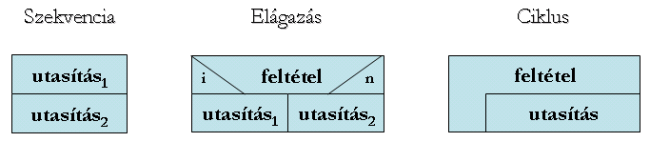
\includegraphics[width=0.7\linewidth]{img/stuki_alapszerk1}
			\caption{A struktogram összetett alapszerkezetei.}
			\label{fig:stuki_alapszerk1}
		\end{figure}

	Szekvenciánál a téglalapok egymás alatti sorrendje dönti el a végrehajtás sorrendjét. Az elágazásfeltétel igaz értéke esetén az i betűvel jelölt bal oldali téglalap utasítását kell végrehajtani, hamis értéke esetén pedig az n betűvel jelölt jobb oldali téglalapét. Ha az elágazás valamelyik ága üres, akkor a neki megfelelő téglalap is üres marad. A ciklus elöltesztelős, azaz a benne levő utasítást mindaddig végre kell hajtani, amíg a feltétel igaz.
	
	Az utasítások helyén lehet egyetlen elemi utasítás, lehet a három algoritmikus szerkezet valamelyike, és lehet egy eljáráshívás. Ezt a leíróeszközt még többféle elemmel szokták bővíteni: az eljárásdefinícióval, a sokirányú elágazással, illetve a hátultesztelős ciklussal.
	
		\begin{figure}[H]
			\centering
			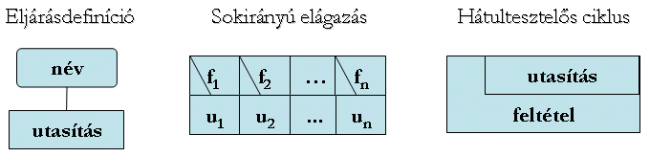
\includegraphics[width=0.7\linewidth]{img/stuki_alapszerk2}
			\caption{A struktogram további összetett alapszerkezetei.}
			\label{fig:stuki_alapszerk2}
		\end{figure}
	
	\noindent Sokirányú elágazásnál azt az ágat kell végrehajtani, amelynek igaz értékű a feltétele (közülük minden esetben pontosan egy teljesülhet).\\
	
	\noindent A lokális adatokat az eljárások téglalapjai mellett, az eljárásnév után sorolhatjuk fel.\\
	
	\noindent Nézzük meg ezzel az eszközzel leírva a következő példát!\\
	
	\noindent Feladat: N tanuló év végi átlagának ismeretében adjuk meg a jeles átlagú tanulók számát!
	
		\begin{figure}[H]
			\centering
			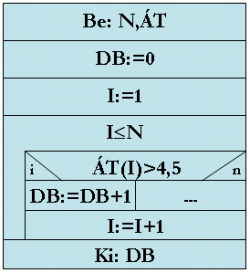
\includegraphics[width=0.4\linewidth]{img/stuki_pelda}
			\caption{A példafeladat megoldása struktogrammal.}
			\label{fig:stuki_pelda}
		\end{figure}
	
	\subsection{Megvalósítás}
	
		A.k.a. kódolás.
	\subsection{Tesztelés}
		A tesztelés célja, hogy minél több hibát megtaláljunk a programban. Ahhoz, hogy az összes hibát fölfedezzük, kézenfekvőnek tűnik a programot kipróbálni az összes lehetséges bemenő adattal. Ez azonban sajnos nem lehetséges.
		
		\noindent Példaként tekintsük a következő - pszeudokóddal megadott - egyszerű programot:
		
		\begin{verbatim}
		Program:
		    Változó A,B:Egész
		   	Be: A,B
		    Ki: A/B
		Program vége.
		\end{verbatim}
		
	Mivel $2^{16}$ különböző értékű egész számot tudunk tárolni, ezért az összes lehetőség $2^{32}$, aminek a leírásához már 9 számjegyre van szükség. Ez rengeteg időt venne igénybe, így nem is járható út.
	
	Ha ezt a programot olyan bemenő adatokkal próbáljuk ki, amelyben A=0 vagy B=1, akkor a program helyesen működik, a hibát nem tudjuk felfedezni. Ezután azt gondolhatnánk, hogy reménytelen helyzetbe kerültünk: hiszen minden lehetséges adattal nem tudjuk kipróbálni a programot; ha pedig kevesebbel próbáljuk ki, akkor lehet, hogy nem vesszük észre a hibákat. A helyzet azért nem ennyire rossz: célunk csak az lehet, hogy a tesztelést olyan módszerrel hajtsuk végre, amellyel a próbák száma erősen lecsökkenthető.\\
	
	Tesztesetnek a be- és kimeneti adatok és feltételek együttes megadását nevezzük. Akkor tudunk a tesztelés eredményeiről bármit is mondani, ha van elképzelésünk arról, hogy adott bemenő adatra milyen eredményt várunk.\\
	
	\noindent Fogalmazzuk meg a tesztelés alapelveit:
	\begin{itemize}
		\item 	A jó teszteset az, ami nagy valószínűséggel egy még felfedetlen hibát mutat ki a programban. Például két szám legnagyobb közös osztóját számoló programot az [5,5] adatpár után a [6,6]-tal teljesen felesleges kipróbálni (ugyanis igencsak rafinált, valószínűtlen elírás esetén viselkedhet a program [6,6]-ra másként, mint [5,5]-re).
	
		\item 	A teszteset nemcsak bemenő adatokból, hanem a hozzájuk tartozó eredményekből is áll. Egyébként nem tudnánk a kapott eredmény helyes vagy hibás voltáról beszélni. A későbbi felhasználás miatt célszerű a teszteseteket is leírni a fejlesztői dokumentációban vagy egy önálló tesztelési jegyzőkönyvben.
	
		\item	A meg nem ismételhető tesztesetek kerülendők, feleslegesen megnövelik a program-tesztelés költségeit, idejét. Nem is beszélve arról a bosszúságról, amikor a programunk egy hibás futását nem tudjuk megismételni, és így a hiba is felfedetlen marad.
		
		\item	Teszteseteket mind az érvénytelen, mind az érvényes adatokra kell készíteni.
		
		\item 	Minden tesztesetből a lehető legtöbb információt "ki kell bányászni”, azaz minden teszteset eredményét alaposan végig kell vizsgálni. Ezzel jelentősen csökkenthető a szükséges próbák száma.
		
		\item	Egy próba eredményeinek vizsgálata során egyaránt fontos megállapítani, hogy miért nem valósít meg a program valamilyen funkciót, amit elvárunk tőle, illetve hogy miért végez olyan tevékenységeket is, amelyeket nem feltételeztünk róla.
	
		\item	A program tesztelését csak a program írójától különböző személy képes hatékonyan elvégezni. Ennek oka, hogy a tesztelés nem "jóindulatú” tevékenység, saját munkájának vizsgálatához mindenki úgy áll hozzá, hogy önkéntelenül jónak feltételezi.
	\end{itemize}
	
	A programtesztelés módszereit két csoportba oszthatjuk aszerint, hogy a tesztelés során végrehajtjuk-e a programot, vagy nem. Ha csak a program kódját vizsgáljuk, akkor statikus (erről nem esik több szó), ha a programot végre is hajtjuk a tesztelés során, akkor dinamikus tesztelésről beszélünk.
	
	\paragraph{Dinamikus tesztelési módszerek}
	 A dinamikus tesztelési módszerek alapelve az, hogy a programot működés közben vizsgáljuk. Teszteseteket kétféle módon tudunk választani. Egy lehetőség az ún. feketedoboz-módszer, más néven adatvezérelt tesztelés. E módszer alkalmazásakor a tesztelő nem veszi figyelembe a program belső szerkezetét, pontosabban nem azt tekinti elsődleges szempontnak, hanem a teszteseteket a feladat meghatározás alapján választja meg.
	 
	 A cél természetesen a lehető leghatékonyabb tesztelés elvégzése, azaz az összes hiba megtalálása a programban. Ez ugyan elvileg lehetséges, kimerítő bemenet tesztelést kell végrehajtani, a programot ki kell próbálni az összes lehetséges bemenő adatra. Ezzel a módszerrel azonban, mint korábban láttuk, mennyiségi akadályba ütközhetünk.
	 
	 Egy másik lehetőség a fehérdoboz-módszer (logika vezérelt tesztelés). Ebben a módszerben a tesztesetek megválasztásánál lehetőség van a program belső szerkezetének figyelembevételére is.
	 
	 A cél a program minél alaposabb tesztelése, erre jó módszer a kimerítő út tesztelés. Ez azt jelenti, hogy a programban az összes lehetséges utat végigjárjuk, azaz annyi tesztesetet hozunk létre, hogy ezt elérhessük vele. Az a probléma, hogy még viszonylag kis programok esetén is igen nagy lehet a tesztelési utak száma. Gondoljunk a ciklusokra! Sőt ezzel a módszerrel a hiányzó utakat nem lehet felderíteni.
	 
	 Mivel sem a fehérdoboz-módszerrel, sem a feketedoboz-módszerrel nem lehetséges a kimerítő tesztelés, el kell fogadnunk, hogy nem tudjuk egyetlen program hibamentességét sem szavatolni. A további cél ezek után az összes lehetséges teszteset halmazából a lehető leghatékonyabb teszteset-csoport kiválasztása lehet.
	 
	 A tesztelés hatékonyságát kétféle jellemző határozza meg: a tesztelés költsége és a felfedett hibák aránya. A leghatékonyabb teszteset-csoport tehát minimális költséggel maximális számú hibát fed fel.
	 
	 A feketedoboz- és fehérdoboz-teszteken kívül még érdemes megemlíteni olyan speciális teszteket, amikor nem a helyesség belátása a cél. Ilyen pl. a stresszteszt (nagy adatmennyiséget hogyan bír kezelni a program, jól skálázódik-e) vagy a hatékonysági teszt (végrehajtási idő tesztelése).
	 
	\section{Az adattípus fogalma}
	
	\subsection{Alapfogalmak, jelölések}
	
	\begin{itemize}
	
		\item	$A^{*}$ az A-beli véges sorozatok halmazát, $A^{\infty}$ az A-beli végtelen sorozatok halmazát jelöli.
		A kettő uniója $A^{**} = A^{*} \cup A^{\infty}$ pedig az A-beli véges vagy végtelen sorozatok halmazát jelenti.
	
		\item	Legyen $R \subseteq A \times \mathbb{L}$ egy logikai reláció. Ekkor az R igazsághalmaza
		$\lceil R \rceil ::= R^{-1}(\left\{{igaz}\right\}) $
		
		\item	Legyen I egy véges halmaz és legyenek $A_{i}, i \in I$ tetszőlege véges vagy megszámolható, nem üres halmazok.
		Ekkor az $A = \underset{i \in I}{\times} A_{i}$ halmazt állapottérnek, az $A_{i}$ halmazokat pedig típusértékhalmazoknak nevezzük.
		
		\item	Feladat: feladatnak nevezünk egy $F \subseteq A \times A$ relációt.\\
		A feladat fenti definíciója természetes módon adódik abból, hogy a feladatot egy
		leképezésnek tekintjük az állapottéren, és az állapottér minden pontjára megmondjuk,
		hova kell belőle eljutni, ha egyáltalán el kell jutni belőle valahova.
		
		\item Program:\\
		Programnak nevezzük az $S \subseteq A \times A^{**}$ relációt, ha
			\begin{enumerate}
				\item	$\mathcal{D}_{S}=A$ (az állapottér minden pontjához rendel valamit, azaz a program minden pontban csinál valamit)
				\item	$\forall \alpha \in \mathcal{R}_{S} : \alpha = red(\alpha)$ (az állapot megváltozik, vagy ha mégsem, az az abnormális működés jele)
				\item	$\forall a \in A : \forall \alpha \in S(A) : |\alpha| \not = 0$ és $\alpha_{1}=a$
			\end{enumerate}
		\noindent A fenti definícióval a "működés” fogalmát akarjuk absztrakt módon megfogalmazni.
		
	\end{itemize}
	
	\subsection{Típusspecifikáció}
			
	Először bevezetünk egy olyan fogalmat, amelyet arra használhatunk, hogy pontosan
	leírjuk a követelményeinket egy típusértékhalmazzal és a rajta végezhető
	műveletekkel szemben.\\
	
	\noindent A $\mathcal{T_{S}}=(H,I_{S},\mathbb{F})$ hármast típusspecifikációnak nevezzük, ha
	teljesülnek rá a következő feltételek:
	
	\begin{enumerate}
		\item H az alaphalmaz,
		
		\item $I_{S} : H \to \mathbb{L} $ a specifikációs invariáns,
	
		\item $T_{\mathcal{T}} = \left\{ {(\mathcal{T},x) | x \in \lceil I_{S}} \rceil\right\}$ a típusértékhalmaz,
		
		\item $\mathbb{F} = \left\{ {F_{1},F_{2},...,F_{n}}\right\}$ a típusműveletek specifikációja, ahol\\
		$\forall i \in [1..n]: F_{i} \subseteq A_{i} \times A_{i}$, $A_{i} = A_{i_{1}} \times ... \times A_{i_{n_{i}}}$ úgy,\\
		hogy $\exists j \in [1..n_{i}]: A_{i_{j}} = T_{\mathcal{T}} $
	\end{enumerate}
	
	Az alaphalmaz és az invariáns tulajdonság segítségével azt fogalmazzuk meg,
	hogy mi az a halmaz, $T_{\mathcal{T}}$, amelynek elemeivel foglalkozni akarunk, míg a feladatok
	halmazával azt írjuk le, hogy ezekkel az elemekkel milyen műveletek végezhetők
	el.
	
	Az állapottér definíciójában szereplő típusértékhalmazok mind ilyen típusspecifikációban
	vannak definiálva. Az állapottér egy komponensét egy program csak a típusműveleteken keresztül változtathatja meg.
	\subsection{Típus}

	Vizsgáljuk meg, hogy a típusspecifikációban leírt követelményeket hogyan valósítjuk
	meg.\\
	
	\noindent A $\mathcal{T}=(\rho,I,\mathbb{S})$ hármast típusnak nevezzük, ha

	\begin{enumerate}
		\item $\rho \subseteq E^{*} \times T$ a reprezentációs függvény (reláció),\\
		T a típusértékhalmaz,\\
		E az elemi típusértékhalmaz
		\item $I : E^{*} \to \mathbb{L} $ típusinvariáns
		\item $\mathbb{S} = \left\{ {S_{1},S_{2},...,S_{m}}\right\}$, ahol\\
		$\forall i \in [1..m]: S_{i} \subseteq B_{i} \times B_{i}^{**}$ program, $B_{i} = B_{i_{1}} \times ... \times B_{i_{m_{i}}}$ úgy,\\
		hogy $\exists j \in [1..m_{i}]: B_{i_{j}} = E^{*}$ és $\not \exists j \in [1..m_{i}]: B_{i_{j}} = T$
	\end{enumerate}
	
	A típus első két komponense az absztrakt típusértékek reprezentációját írja le, míg a programhalmaz a típusműveletek implementációját tartalmazza. Az elemi típusértékhalmaz lehet egy tetszőleges másik típus típusértékhalmaza vagy egy, valamilyen módon definiált legfeljebb megszámolható halmaz.
	
	\subsection{Invariáns}
	
	Az invariáns lényege, hogy ezt a tulajdonságot soha nem sérthetjük meg. Például halmaz típus esetén nem szabad, hogy megsérüljön
	az az invariáns tulajdonság, hogy egy halmazban egy elem csak egyszer fordulhat elő.
	
	\subsection{Reprezentáció}
	
	Azt, hogy egy típust milyen típusok segítségével, milyen módszerrel, stb., valósítottunk meg, reprezentációnak nevezzük. Például
	egy verem típust meg lehet valósítani tömb segítségével, de láncolt listával is.
	
	A reprezentáció a típusspecifikáció típusértékhalmazának leképezése a konkrét típusban, amit a reprezentációs függvény ad meg.
	
	\subsection{Implementáció}
	
	Az implementáció a típusspecifikáció típusműveleteinek megvalósítása a konkrét típus programhalmaza által.
	
	Az implementáció során a típus megvalósításakor a típusértékhalmaz megadását követően definiálni kell a típusműveleteket. Ahogyan a modellben is, a gyakorlatban is az állapottér változásait a program csak a típusműveleteken keresztül végezheti el.
	
	\subsection{Emészthetőbb módon}
	
	\begin{figure}[H]
		\centering
		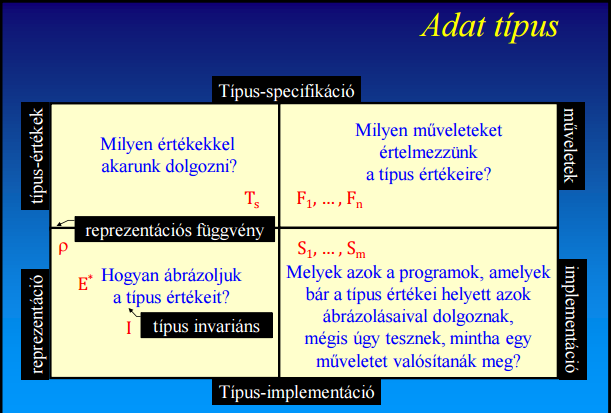
\includegraphics[width=0.7\linewidth]{img/adattipus}
		\caption{Adattípus}
		\label{fig:adattipus}
	\end{figure}

	\begin{figure}[H]
		\centering
		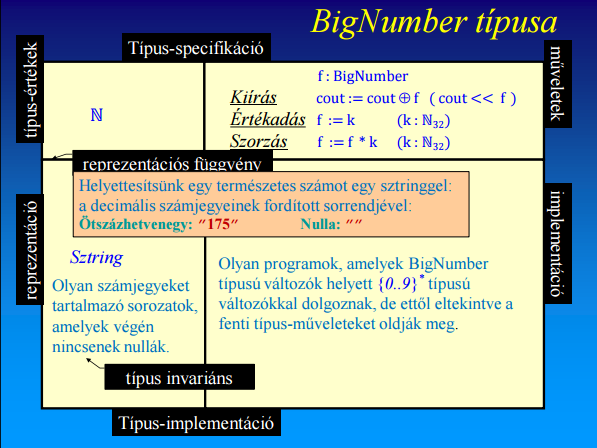
\includegraphics[width=0.7\linewidth]{img/adattipus_pelda}
		\caption{BigNumber példa}
		\label{fig:adattipus_pelda}
	\end{figure}	
	
	\section{A visszavezetés módszere}
	
	A programozási feladatok megoldásához különböző programozási mintákat, ún. programozási tételeket használunk fel, ezekre vezetjük vissza
	a megoldást.\\
	
	\noindent Lépései:
	\begin{enumerate}
		\item	Megsejtjük a feladatot megoldó programozási tételt.
		\item	Specifikáljuk a feladatot a programozási tétel jelöléseivel.
		\item	Megadjuk a programozási tétel és a feladat közötti eltéréseket:
			\begin{itemize}
				\item	intervallum határok: konkrét érték vagy kifejezés (pl. $[1..\frac{n}{2}]$),
				a típusuk a $\mathbb{Z}$ helyett lehet annak valamely része (pl. $\mathbb{N}$)
				
				\item	$\beta:[m..n] \to \mathbb{L}$ és/vagy $f:[m..n] \to H$ konkrét megfelelői
				
				\item	a H megfelelője a szükséges művelettel
					\begin{itemize}
						\item	$(H,>)$ helyett pl. $(\mathbb{Z},>)$ vagy $(\mathbb{Z},<)$
						\item	$(H,+)$ helyett pl. $(\mathbb{Z},+)$ vagy $(\mathbb{R},*)$
					\end{itemize}
				\item	a változók átnevezése
			\end{itemize}
		\item	A különbségek figyelembe vételével a tétel algoritmusából elkészítjük a konkrét feladatot megoldó algoritmust.
	\end{enumerate}
	
	\section{Felsoroló, a felsoroló típus specifikációja}
	
	A gyűjtemény (tároló, kollekció, iterált) egy olyan adat
	(objektum), amely valamilyen elemek tárolására alkalmas.
	\begin{itemize}
		\item	Ilyenek az összetett szerkezetű, de különösen az iterált szerkezetű
		típusok értékei: halmaz, sorozat (verem, sor, fájl), fa, gráf

		\item	De vannak úgynevezett virtuális gyűjtemények is: pl. egész számok
		egy intervallumának elemei, vagy egy természetes szám prím-osztói
	\end{itemize}
	
	\noindent Egy gyűjtemény feldolgozásán a benne levő elemek
	feldolgozását értjük.
	\begin{itemize}
		\item	Keressük a halmaz legnagyobb elemét!
		\item	Hány negatív szám van egy számsorozatban?
		\item	Válogassuk ki egy fa leveleiben elhelyezett értékeket!
		\item	Járjuk be az [m .. n] intervallum minden második elemét visszafelé!
		\item	Adjuk össze az n természetes szám prím-osztóit!
	\end{itemize}
	
	\noindent A feldolgozni kívánt elemek felsorolását (bejárását) az alábbi
	műveletekkel szabványosítjuk:
	\begin{itemize}
		\item	First() : Rááll a felsorolás első elemére, azaz elkezdi a felsorolást
		\item	Next() : Rááll az elkezdett felsorolás soron következő elemére
		\item	End() : Mutatja, ha a felsorolás végére értünk
		\item	Current() : Visszaadja a felsorolás aktuális elemét
	\end{itemize}
	
	Egy felsorolásnak különböző állapotai vannak (indulásra kész,
	folyamatban van, befejeződött), és a műveletek csak bizonyos
	állapotokban értelmezhetők (máshol a hatásuk nem definiált). 
	A feldolgozó algoritmus garantálja,	hogy a felsoroló műveletek mindig
	megfelelő állapotban kerüljenek	végrehajtásra.

	\begin{figure}[H]
		\centering
		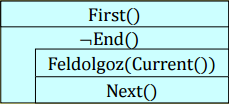
\includegraphics[width=0.4\linewidth]{img/felsorolas_stuki}
		\caption{A felsorolás algoritmusa}
		\label{fig:felsorolas_stuki}
	\end{figure}
	
	A felsorolást sohasem a felsorolni kívánt gyűjtemény, hanem
	egy külön felsoroló objektum végzi. 

	\begin{figure}[H]
		\centering
		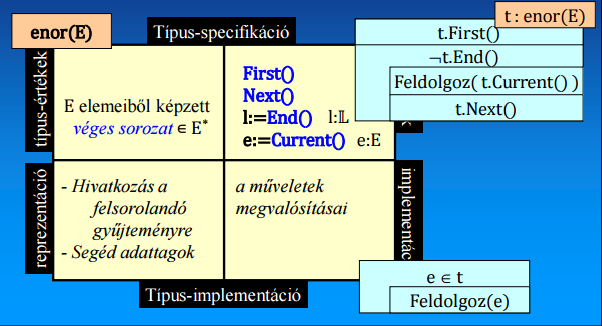
\includegraphics[width=0.7\linewidth]{img/felsorolo_speci}
		\caption{A felsoroló objektum és típusa}
		\label{fig:felsorolas_stuki}
	\end{figure}
	
	\section{Felsorolóra megfogalmazott programozási tételek}
	
	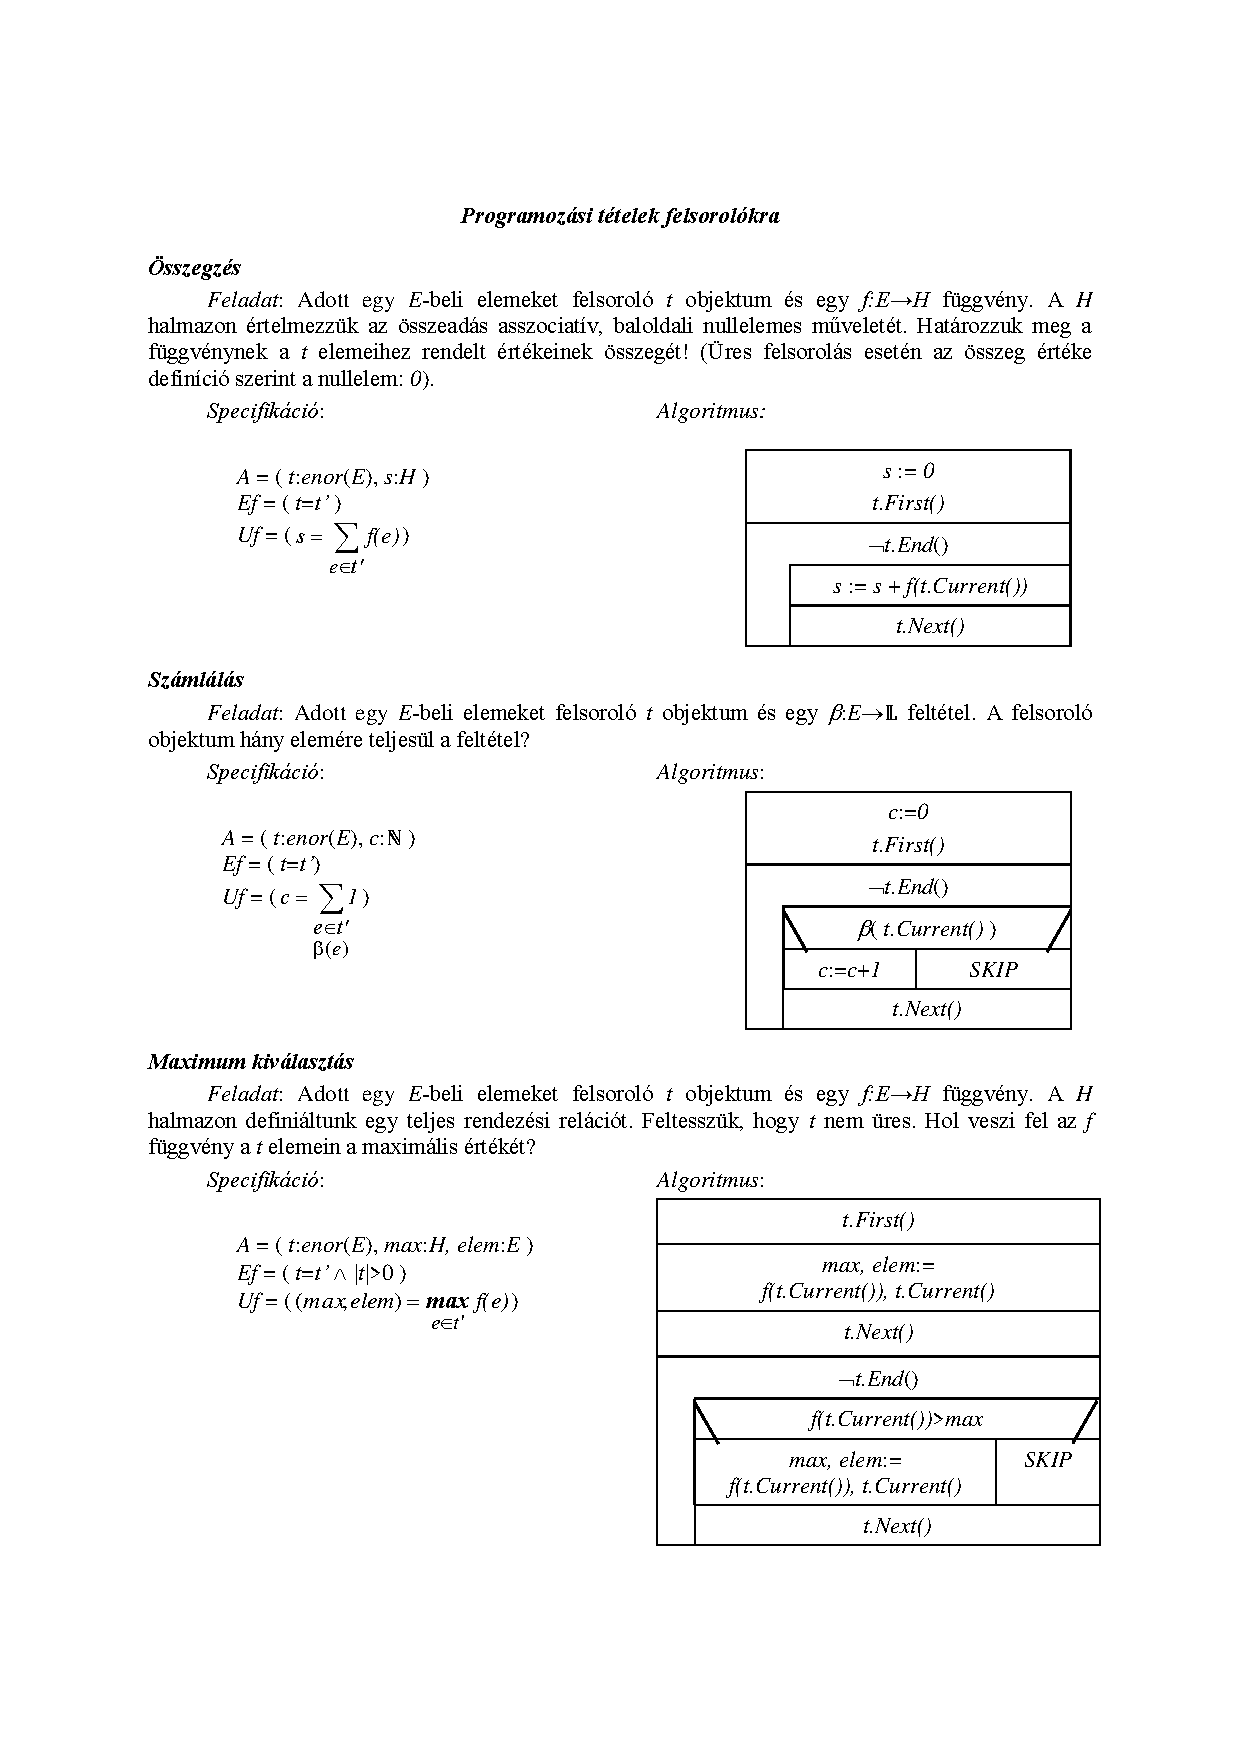
\includepdf[pages={1-2}]{progtetel_felsorolo.pdf}
	
	\section{Nevezetes gyűjtemények felsorolói}
	
	\subsection{Intervallum}
		\begin{figure}[H]
			\centering
			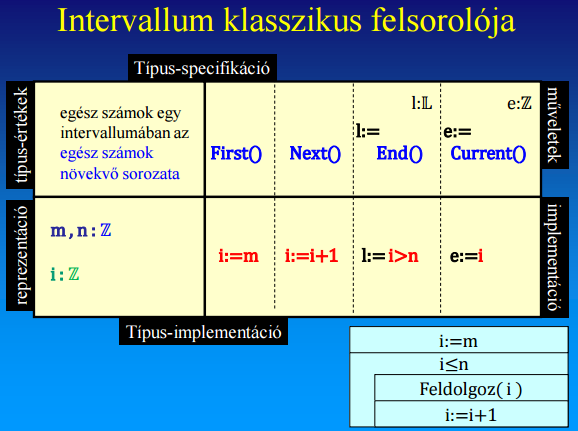
\includegraphics[width=0.7\linewidth]{img/felsorolo_intervallum}
			\caption{Intervallum felsorolója}
			\label{fig:felsorolo_intervallum}
		\end{figure}
	
	\subsection{Tömb}
	Itt két különböző tömbtípus felsorolóját mutatjuk be: az egydimenziós (vektor) és a kétdimenziós tömbét (mátrix).
	
	\begin{figure}[H]
		\centering
		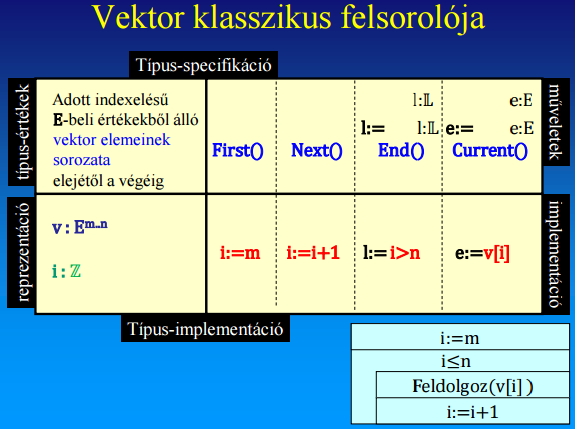
\includegraphics[width=0.7\linewidth]{img/felsorolo_vektor}
		\caption{Vektor felsorolója}
		\label{fig:felsorolo_vektor}
	\end{figure}
	
	\begin{figure}[H]
		\centering
		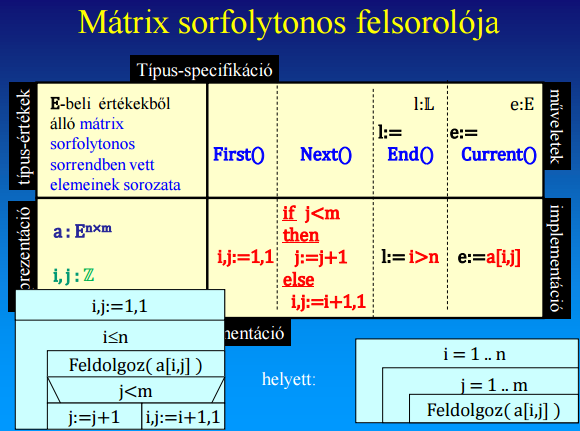
\includegraphics[width=0.7\linewidth]{img/felsorolo_matrix}
		\caption{Mátrix sorfolytonos felsorolója}
		\label{fig:felsorolo_matrix}
	\end{figure}
	
	Megjegyzés: a felsorolás történhet másképpen is, például vektor esetén végezhetjük a felsorolást visszafelé, a tömb végétől kezdve, vagy mátrixnál alkalmazhatunk pl. oszlopfolytonos bejárást.
	
	\subsection{Sorozat}
		\begin{figure}[H]
			\centering
			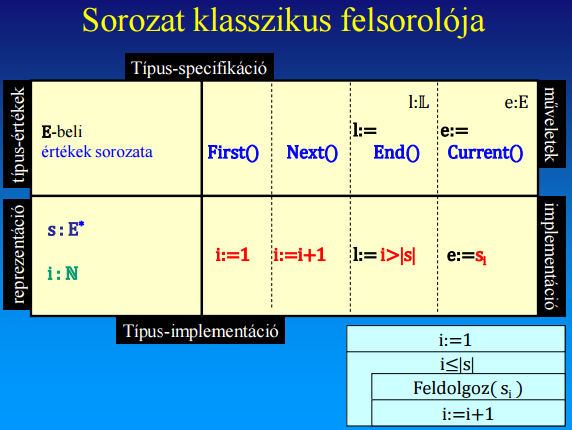
\includegraphics[width=0.7\linewidth]{img/felsorolo_sorozat}
			\caption{Sorozat felsorolója}
			\label{fig:felsorolo_sorozat}
		\end{figure}

	\subsection{Halmaz}
		\begin{figure}[H]
			\centering
			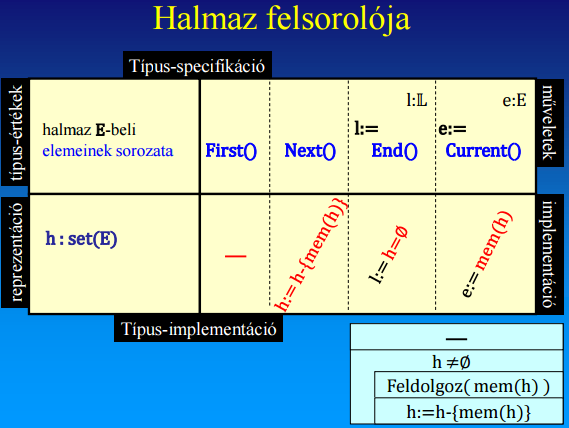
\includegraphics[width=0.7\linewidth]{img/felsorolo_halmaz}
			\caption{Halmaz felsorolója}
			\label{fig:felsorolo_halmaz}
		\end{figure}

	\subsection{Szekvenciális inputfájl}
		\begin{figure}[H]
			\centering
			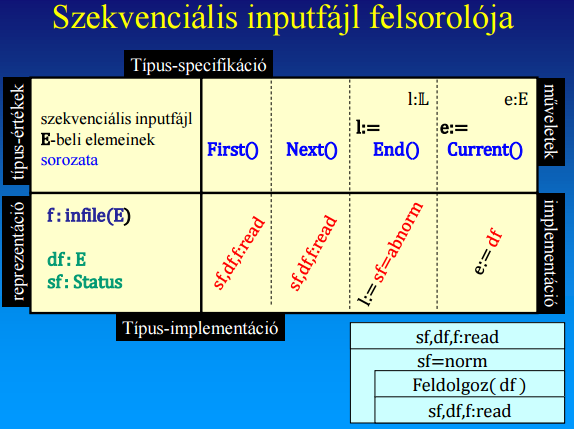
\includegraphics[width=0.7\linewidth]{img/felsorolo_seqin}
			\caption{Szekvenciális inputfájl felsorolója}
			\label{fig:felsorolo_seqin}
		\end{figure}
	
\end{document}